\documentclass[11pt]{article}
\usepackage[margin=1in]{geometry}
\usepackage{amsmath, amssymb, amsthm}
\usepackage{tikz}
\usepackage{mdframed}
\usepackage{listing}

% Define custom environments for a professional notebook layout
\newtheorem{problem}{Exercise}

\begin{document}
	
	% ---------------------------------------------------------
	% COVER PAGE
	% ---------------------------------------------------------
	\begin{titlepage}
		\centering
		\vspace*{4cm}
		
		{\Huge \textbf{Riemann Surface \& Algebraic Curve Theory}} \\
		\vspace{0.5cm}
		{\Large \textbf{for understanding Elliptic Curve}} \\
		
		\vspace{2cm}
		
		{\Large \textit{Practice Problems:}} \\
		\vspace{0.2cm}
		{\huge \textbf{Goppa Codes and Integrals of Winding Forms}}
		
		\vfill
		
		% Optional: Add author or date here
		{\large \today}
	\end{titlepage}
	
	% ---------------------------------------------------------
	% EXERCISE 1
	% ---------------------------------------------------------
	\newpage
	\thispagestyle{plain}
	
	\begin{problem}[The Local Winding Form and Coordinate Extraction]
		Let $\mathbb{P}^1(\mathbb{C})$ be the Riemann sphere. Define a set of distinct support points $L = \{a_1, a_2, \dots, a_n\} \subset \mathbb{C}$. Let $c = (c_1, \dots, c_n) \in \mathbb{C}^n$ be a vector over the complex numbers. 
		
		Define the global meromorphic winding form associated with $c$ as:
		$$ \omega_c = \sum_{i=1}^n c_i \frac{dz}{z - a_i} $$
		
		Let $\gamma_j$ be a small, counterclockwise closed contour enclosing $a_j$ but no other points of the support set $L$. Prove, using Cauchy's Integral Formula, that the local contour integral over $\gamma_j$ strictly extracts the $j$-th coordinate of the vector $c$.
	\end{problem}
	
	\vspace{0.5cm}
	
	\begin{mdframed}[backgroundcolor=gray!5, linecolor=gray!50, linewidth=1pt]
		\textbf{Solution Space:}
		
		% TikZ Placeholder for Exercise 1
		\begin{center}
			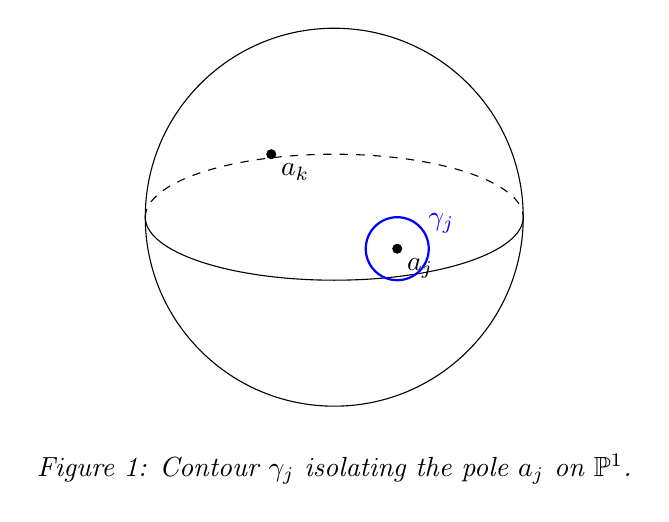
\begin{tikzpicture}[scale=0.8]
				% Draw the Riemann sphere boundary
				\draw (0,0) circle (3cm);
				\draw[dashed] (-3,0) arc (180:0:3cm and 1cm);
				\draw (-3,0) arc (180:360:3cm and 1cm);
				
				% Draw poles and contours
				\filldraw (1,-0.5) circle (2pt) node[below right] {$a_j$};
				\draw[->, thick, blue] (1,-0.5) circle (0.5cm);
				\node[blue] at (1.7,-0.1) {$\gamma_j$};
				
				\filldraw (-1, 1) circle (2pt) node[below right] {$a_k$};
				
				\node at (0, -4) {\textit{Figure 1: Contour $\gamma_j$ isolating the pole $a_j$ on $\mathbb{P}^1$.}};
			\end{tikzpicture}
		\end{center}
		
		\vspace{0.5cm}
		\textit{(Student proof begins here...)}
		
	\end{mdframed}
	
	% ---------------------------------------------------------
	% EXERCISE 2
	% ---------------------------------------------------------
	\newpage
	\thispagestyle{plain}
	
	\begin{problem}[The Holomorphic Constraint and the Goppa Polynomial]
		Let $g(z)$ be a Goppa polynomial of degree $t$, whose roots are completely disjoint from the support set $L$. We constrain our vector space by requiring that the winding form $\omega_c$ has a zero of multiplicity at least $1$ wherever $g(z)$ has a root.
		
		Let $h(z)$ be any arbitrary test polynomial of degree strictly less than $t$. Define a new differential form:
		$$ \eta = h(z) \omega_c $$
		
		Show that if $\omega_c$ satisfies the Goppa zero-constraint, the new differential form $\eta$ is guaranteed to be holomorphic (analytic and pole-free) at the roots of $g(z)$, meaning all poles of $\eta$ are strictly confined to the support set $L$.
	\end{problem}
	
	\vspace{0.5cm}
	
	\begin{mdframed}[backgroundcolor=gray!5, linecolor=gray!50, linewidth=1pt]
		\textbf{Solution Space:}
		
		\vspace{0.5cm}
		\textit{(Student proof begins here...)}
		
	\end{mdframed}
	
	% ---------------------------------------------------------
	% EXERCISE 3
	% ---------------------------------------------------------
	\newpage
	\thispagestyle{plain}
	
	\begin{problem}[Stokes' Theorem and the Parity-Check Kernel]
		Consider the compact manifold $M$ formed by taking the Riemann sphere $\mathbb{P}^1$ and removing small open disks around each point $a_i \in L$. The boundary $\partial M$ of this manifold consists of all the contour loops from Exercise 1, oriented clockwise (denoted $-\gamma_i$).
		
		Apply the Global Residue Theorem (a consequence of the generalized Stokes' Theorem, $\int_{\partial M} \eta = \iint_M d\eta$) to the differential form $\eta = h(z) \omega_c$ from Exercise 2. 
		
		Prove that for any test polynomial $h(z)$ of degree less than $t$, the coordinates $c_i$ must satisfy the global integral constraint:
		$$ \sum_{i=1}^n c_i h(a_i) = 0 $$
		\textit{Hint: Conclude by explaining how iterating $h(z)$ through the basis $\{1, z, z^2, \dots, z^{t-1}\}$ constructs the classical parity-check matrix $H$, proving the code is a well-defined kernel.}
	\end{problem}
	
	\vspace{0.5cm}
	
	\begin{mdframed}[backgroundcolor=gray!5, linecolor=gray!50, linewidth=1pt]
		\textbf{Solution Space:}
		
		% TikZ Placeholder for Exercise 3
		\begin{center}
			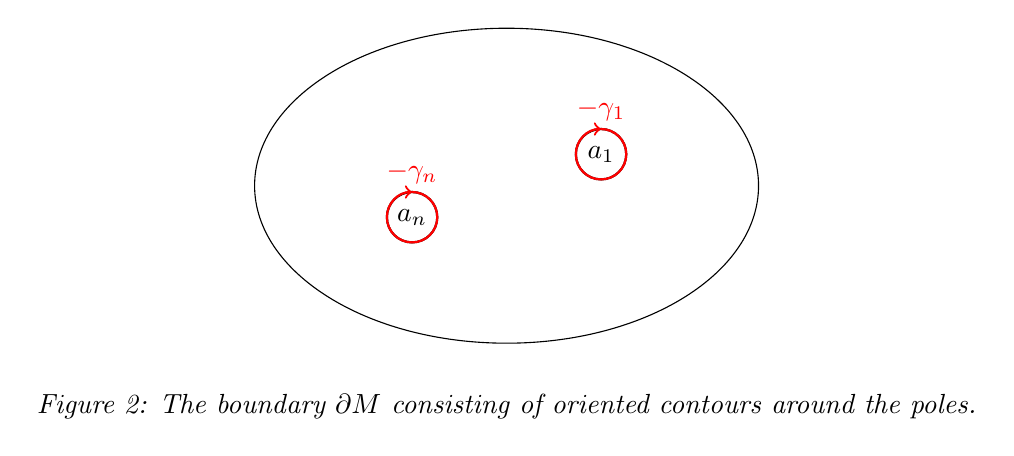
\begin{tikzpicture}[scale=0.8]
				% Draw the manifold with holes
				\draw (0,0) ellipse (4cm and 2.5cm);
				
				% Draw holes with clockwise orientation
				\filldraw[fill=white, draw=black, thick] (1.5, 0.5) circle (0.4cm);
				\draw[<-, thick, red] (1.5, 0.9) arc (90:450:0.4cm);
				\node[red] at (1.5, 1.2) {$-\gamma_1$};
				\node at (1.5, 0.5) {$a_1$};
				
				\filldraw[fill=white, draw=black, thick] (-1.5, -0.5) circle (0.4cm);
				\draw[<-, thick, red] (-1.5, -0.1) arc (90:450:0.4cm);
				\node[red] at (-1.5, 0.2) {$-\gamma_n$};
				\node at (-1.5, -0.5) {$a_n$};
				
				\node at (0, -3.5) {\textit{Figure 2: The boundary $\partial M$ consisting of oriented contours around the poles.}};
			\end{tikzpicture}
		\end{center}
		
		\vspace{0.5cm}
		\textit{(Student proof begins here...)}
		
	\end{mdframed}


	\newpage
	
	\begin{center}
		{\Huge \textbf{Solutions Manual}} \\
		\vspace{0.3cm}
		{\Large \textit{Goppa Codes and Integrals of Winding Forms}}
	\end{center}
	
	\vspace{1cm}
	
	% ---------------------------------------------------------
	% SOLUTION 1
	% ---------------------------------------------------------
	\begin{problem}[The Local Winding Form and Coordinate Extraction]
		% Problem statement omitted for brevity in the solutions manual
	\end{problem}
	
	\begin{mdframed}[backgroundcolor=gray!5, linecolor=gray!50, linewidth=1pt]
		\textbf{Proof:}
		
		By definition, the global meromorphic winding form is:
		$$ \omega_c = \sum_{i=1}^n c_i \frac{dz}{z - a_i} $$
		
		We integrate $\omega_c$ along the closed contour $\gamma_j$, which encloses $a_j$ but no other points of the support set $L$:
		$$ \frac{1}{2\pi i} \oint_{\gamma_j} \omega_c = \frac{1}{2\pi i} \oint_{\gamma_j} \left( \sum_{i=1}^n c_i \frac{dz}{z - a_i} \right) $$
		
		Because the contour integral is a linear operator, we can distribute the integral inside the finite sum:
		$$ \sum_{i=1}^n c_i \left( \frac{1}{2\pi i} \oint_{\gamma_j} \frac{dz}{z - a_i} \right) $$
		
		By Cauchy's Integral Formula (or the Residue Theorem), the integral of $\frac{dz}{z - a_i}$ along $\gamma_j$ evaluates to $1$ if $i = j$ (since $a_j$ is inside $\gamma_j$) and $0$ if $i \neq j$ (since $a_i$ is outside $\gamma_j$ and the integrand is holomorphic there). This acts as the Kronecker delta $\delta_{ij}$:
		$$ \sum_{i=1}^n c_i \delta_{ij} = c_j $$
		
		Thus, the contour integral strictly extracts the coordinate $c_j$, proving the mapping from the continuous differential space to the discrete vector space $\mathbb{C}^n$ is perfectly well-defined. \hfill $\blacksquare$
	\end{mdframed}
	
	\vspace{1cm}
	
	% ---------------------------------------------------------
	% SOLUTION 2
	% ---------------------------------------------------------
	\begin{problem}[The Holomorphic Constraint and the Goppa Polynomial]
	\end{problem}
	
	\begin{mdframed}[backgroundcolor=gray!5, linecolor=gray!50, linewidth=1pt]
		\textbf{Proof:}
		
		Let $\beta$ be a root of the Goppa polynomial $g(z)$. By the established constraint, the winding form $\omega_c$ must have a zero of multiplicity $m \geq 1$ at $z = \beta$. 
		
		Therefore, in a local neighborhood around $\beta$, we can write $\omega_c$ as:
		$$ \omega_c = (z - \beta)^m \phi(z) dz $$
		where $\phi(z)$ is a locally holomorphic function such that $\phi(\beta) \neq 0$.
		
		Let $h(z)$ be an arbitrary polynomial. Because polynomials are entire functions, $h(z)$ is holomorphic everywhere on $\mathbb{C}$. 
		
		We evaluate the local structure of the new differential form $\eta = h(z)\omega_c$ near the root $\beta$:
		$$ \eta = h(z) (z - \beta)^m \phi(z) dz $$
		
		Since $h(z)$, $(z-\beta)^m$, and $\phi(z)$ are all holomorphic at $z = \beta$, their product is also holomorphic at $z = \beta$. The multiplication by $h(z)$ cannot introduce any new poles because $h(z)$ is a polynomial. 
		
		Since $\omega_c$ only has poles at the support set $L$, and $h(z)$ introduces no poles and preserves the analyticity at the roots of $g(z)$, the form $\eta$ remains holomorphic everywhere except for isolated simple poles strictly contained within $L$. \hfill $\blacksquare$
	\end{mdframed}
	
	\newpage
	
	% ---------------------------------------------------------
	% SOLUTION 3
	% ---------------------------------------------------------
	\begin{problem}[Stokes' Theorem and the Parity-Check Kernel]
	\end{problem}
	
	\begin{mdframed}[backgroundcolor=gray!5, linecolor=gray!50, linewidth=1pt]
		\textbf{Proof:}
		
		Let $M = \mathbb{P}^1 \setminus \bigcup_{i=1}^n D_i$, where $D_i$ are small open disks around each pole $a_i$. The boundary $\partial M$ consists of the negatively oriented contours $\bigcup_{i=1}^n -\gamma_i$.
		
		We apply the generalized Stokes' Theorem to the differential form $\eta = h(z)\omega_c$:
		$$ \int_{\partial M} \eta = \iint_M d\eta $$
		
		From Exercise 2, $\eta$ is holomorphic everywhere on $M$ (the constraint ensures it is well-behaved at the roots of $g(z)$, and the poles $a_i$ have been removed). Because $\eta$ is a holomorphic 1-form, it is closed, meaning its exterior derivative $d\eta = 0$. Therefore, the area integral vanishes:
		$$ \iint_M d\eta = 0 \implies \int_{\partial M} \eta = 0 $$
		
		Expanding the boundary integral into the sum of the individual contours:
		$$ \sum_{i=1}^n \oint_{-\gamma_i} \eta = 0 \implies \sum_{i=1}^n \frac{1}{2\pi i} \oint_{\gamma_i} h(z)\omega_c = 0 $$
		
		Because $h(z)$ is holomorphic at $a_i$, we can evaluate the residue of $h(z)\omega_c$ at $a_i$. Using the definition of $\omega_c$ from Exercise 1, the residue at $a_i$ is simply $c_i h(a_i)$. Substituting this into the sum yields the global constraint:
		$$ \sum_{i=1}^n c_i h(a_i) = 0 $$
		
		\textbf{Constructing the Kernel:} \\
		To form the parity-check matrix $H$, we let the test polynomial $h(z)$ range over the basis of polynomials of degree less than $t$: $\{1, z, z^2, \dots, z^{t-1}\}$. 
		Evaluating the constraint for $h(z) = z^k$ gives the equation:
		$$ \sum_{i=1}^n c_i a_i^k = 0 \quad \text{for } k = 0, 1, \dots, t-1 $$
		This generates exactly $t$ linear equations. The code is therefore the rigorously well-defined nullspace of the $t \times n$ matrix $H$ where $H_{k,i} = a_i^k$. \hfill $\blacksquare$
	\end{mdframed}

	\newpage
	\begin{center}
		{\Huge \textbf{Appendix}} \\
		\vspace{0.3cm}
		{\Large \textit{The Algebraic-Geometric Bridge}}
	\end{center}
	
	\vspace{1cm}
	
	\begin{mdframed}[backgroundcolor=white, linecolor=black, linewidth=1.5pt, roundcorner=5pt, innerleftmargin=15pt, innerrightmargin=15pt, innertopmargin=15pt, innerbottommargin=15pt]
		
		\textbf{Connecting the Continuous Integral to the Discrete Syndrome}
		
		In classical coding theory textbooks, the Goppa code over a finite field $\mathbb{F}_q$ is defined purely algebraically. A vector $c \in \mathbb{F}_q^n$ is a valid codeword if and only if it satisfies the syndrome equation:
		$$ \sum_{i=1}^n \frac{c_i}{x - a_i} \equiv 0 \pmod{g(x)} $$
		
		How does this discrete modular arithmetic relate to the continuous differential geometry of winding forms and compact Riemann surfaces? They are identically the same constraint, translated from the language of analysis to the language of algebra.
		
		\vspace{0.5cm}
		\textbf{1. The Continuous Perspective (Analytic Zeroes)} \\
		In Exercise 2, we established that the differential form $\omega_c = \sum_{i=1}^n c_i \frac{dz}{z - a_i}$ must have zeroes at the roots of the Goppa polynomial $g(z)$. 
		
		If $\beta$ is a root of $g(z)$ with multiplicity $m$, the analytic function $f(z) = \sum_{i=1}^n \frac{c_i}{z - a_i}$ must have a zero of order at least $m$ at $z = \beta$. In complex analysis, this means the Taylor series expansion of $f(z)$ centered at $\beta$ must look like:
		$$ f(z) = A_m (z - \beta)^m + A_{m+1} (z - \beta)^{m+1} + \dots $$
		Notice that the constant term, the $z-\beta$ term, up to the $(z-\beta)^{m-1}$ term must all be strictly zero.
		
		\vspace{0.5cm}
		\textbf{2. The Algebraic Perspective (Quotient Rings)} \\
		Over a finite field, we cannot take limits or derivatives to compute Taylor series. Instead, we use the algebraic structure of the polynomial ring $\mathbb{F}_q[x]$ and its quotient ring $\mathbb{F}_q[x]/\langle g(x) \rangle$.
		
		By Bezout's identity, because the support elements $a_i$ are distinct from the roots of $g(x)$, the polynomial $(x - a_i)$ is coprime to $g(x)$. Therefore, the term $\frac{1}{x - a_i}$ is not a fraction; it is the unique, rigorously defined multiplicative inverse $(x - a_i)^{-1}$ within the quotient ring.
		
		\vspace{0.5cm}
		\textbf{3. The Grand Equivalence} \\
		To say that $\sum_{i=1}^n c_i (x - a_i)^{-1} \equiv 0 \pmod{g(x)}$ means that when you algebraically expand this sum into a polynomial, it is a perfect multiple of $g(x)$. 
		
		If it is a perfect multiple of $g(x)$, it must contain $(x - \beta)^m$ as a factor for every root $\beta$. Algebraically containing $(x - \beta)^m$ as a factor is the exact, discrete equivalent of a continuous analytic function having its first $m$ Taylor coefficients vanish at $\beta$. 
		
		Therefore, the algebraic parity-check matrix $H$ over a finite field is nothing more than the discretized calculation of the vanishing Taylor series coefficients dictated by the generalized Stokes' Theorem on a compact manifold.
	\end{mdframed}

	\newpage
	\begin{center}
		{\Huge \textbf{Appendix B}} \\
		\vspace{0.3cm}
		{\Large \textit{Algorithmic Verification with SageMath}}
	\end{center}
	
	\vspace{1cm}
	
	\begin{mdframed}[backgroundcolor=white, linecolor=black, linewidth=1.5pt, roundcorner=5pt]
		
		\textbf{Computational Verification of Quotient Ring Inverses}
		
		While theoretical proofs guarantee that $(x - a_i)$ has a unique inverse modulo the Goppa polynomial $g(x)$, practical cryptographic implementations require computing this exact inverse to build the parity-check matrix $H$. 
		
		The following SageMath script demonstrates how to construct the finite field, define the polynomial ring, and algorithmically compute the syndrome fractions using the Extended Euclidean Algorithm under the hood.
		
		\vspace{0.5cm}
		
%\begin{lstlisting}[caption={SageMath implementation for Goppa syndrome inversion}]
%# 1. Define the base field F_2 and the extension field F_8 (2^3)
%F2 = GF(2)
%# We use the irreducible polynomial a^3 + a + 1 = 0
%F8.<a> = GF(2^3, modulus=x^3 + x + 1)
%
%# 2. Define the polynomial ring over the extension field
%R.<x> = PolynomialRing(F8)
%
%# 3. Define the Goppa polynomial g(x) of degree t=2
%g = x^2 + x + a
%
%# 4. Define the quotient ring F_8[x] / <g(x)>
%Q = R.quotient(g, 'X')
%
%# 5. Define a support element a_i (must ensure g(a_i) != 0)
%a_i = a
%print(f"Checking if g(a_i) != 0: {g(a_i) != 0}")
%
%# 6. Compute the inverse of (x - a_i) in the quotient ring
%# We cast (x - a_i) into the quotient ring Q, then invert it
%element = Q(x - a_i)
%inverse_element = element^-1
%
%print(f"The element to invert: {element}")
%print(f"The computed inverse: {inverse_element}")
%
%# 7. Verification
%# Multiplying the element by its inverse should yield 1 modulo g(x)
%identity_check = element * inverse_element
%print(f"Verification (element * inverse): {identity_check}")
%\end{lstlisting}
		
		\vspace{0.5cm}
		\textbf{Understanding the Output}
		
		When this script is executed, SageMath maps the abstract polynomial fraction $\frac{1}{x - a_i}$ directly into the quotient ring. Because $g(a_i) \neq 0$, the elements are coprime, and the `$^-1$` operation securely executes the Extended Euclidean Algorithm over the finite field $\mathbb{F}_{2^3}$ without encountering division-by-zero errors. 
		
		The resulting polynomial $h(x) = h_0 + h_1 x + \dots + h_{t-1} x^{t-1}$ provides the exact coefficients that form the $i$-th column of the parity-check matrix $H_{q^m}$, which can then be expanded into the binary matrix $H$ used in actual hardware or software encoding.
	\end{mdframed}
	
\end{document}